\documentclass[preprint]{sigplanconf}

% The following \documentclass options may be useful:
%
% 10pt          To set in 10-point type instead of 9-point.
% 11pt          To set in 11-point type instead of 9-point.
% authoryear    To obtain author/year citation style instead of numeric.

\usepackage{amsmath}
\usepackage[T1]{fontenc}
\usepackage[utf8]{inputenc}
\usepackage[unicode=true,hidelinks]{hyperref}
\usepackage{graphicx}

\usepackage{hyperref}
\usepackage{listings}
%\usepackage[scaled]{luximono}


%\usepackage{natbib}

% ----- begin macros

\lstdefinelanguage{Scala}%
{morekeywords={abstract,%
  case,catch,char,class,%
  def,else,extends,final,for,%
  if,import,implicit,%
  match,module,%
  new,null,%
  object,override,%
  package,private,protected,public,%
  for,public,return,super,%
  this,throw,trait,try,type,%
  val,var,%
  with,%
  yield,%
  lazy%
  },%
  sensitive,%
  morecomment=[l]//,%
  morecomment=[s]{/*}{*/},%
  morestring=[b]",%
  morestring=[b]',%
  showstringspaces=false%
}[keywords,comments,strings]%

\lstdefinelanguage{JavaScript}%
{morekeywords={for, var, attributes, class, classend, do, else, empty, endif, endwhile, fail, function,
functionend, if, implements, in, inherit, inout, not, of, operations, out, return,
then, types, while, use},%
  sensitive,%
  morecomment=[l]//,%
  morecomment=[s]{/*}{*/},%
  morestring=[b]",%
  morestring=[b]',%
  showstringspaces=false%
}[keywords,comments,strings]%

\lstset{language=Scala,%
  mathescape=false,%
%  columns=[c]fixed,%
  aboveskip=\smallskipamount,
  belowskip=\smallskipamount,
%  basewidth={0.5em, 0.4em},%
  basicstyle=\ttfamily\small,%
  keywordstyle=\bfseries%\sffamily\bfseries,%
%  keywordstyle=\sffamily\bfseries,%
%  xleftmargin=0.5cm
}

\newcommand{\commentstyle}[1]{\slseries{#1}}
\newcommand{\keywordstyle}[1]{\bfseries{#1}}

\lstnewenvironment{slisting}{\lstset{language=Scala}}{}

\newcommand{\code}[1]{\lstinline[language=Scala,columns=fixed,basicstyle=\ttfamily\small]|#1|}

\def\changemargin#1#2{\list{}{\rightmargin#2\leftmargin#1}\item[]}
\let\endchangemargin=\endlist

%\setlength{\columnseprule}{0.25pt}

%\renewcommand{\note}[1]{$\spadesuit$ \textbf{#1} $\clubsuit$}


%\newcommand{\comment}[1]{}


\newcommand{\ie}{\emph{i.e.}}
\newcommand{\eg}{\emph{e.g.}}
\newcommand{\cf}{\emph{cf.~}}
\newcommand{\etal}{\emph{et al.~}}
\newcommand{\etc}{\emph{etc.}}
\newcommand{\aka}{\emph{a.k.a.}}


\begin{document}

\conferenceinfo{GPCE '13}{October 27--28, 2013, Indianapolis, Indiana, USA} 
\copyrightyear{2013}
\copyrightdata{[to be supplied]} 

\titlebanner{banner above paper title}        % These are ignored unless
\preprintfooter{short description of paper}   % 'preprint' option specified.

\title{How to build an homogeneous language for heterogeneous platforms}
\subtitle{You don’t have to trade abstraction for control}

\authorinfo{Julien Richard-Foy\and Olivier Barais\and Jean-Marc Jézéquel}
           {IRISA, Université de Rennes 1}
           {\{firstname\}.\{lastname\}@irisa.fr}

\maketitle

\begin{abstract}
This is the text of the abstract.
\end{abstract}

\category{CR-number}{subcategory}{third-level}

\terms
term1, term2

\keywords
keyword1, keyword2

\section{Introduction}

Web applications are attractive because they require no installation or deployment steps on clients and enable large
scale collaborative experiences. However, writing large Web applications is known to be
difficult~\cite{Mikkonen08_SpaghettiJs,Preciado05_RIAMethodologyNecessity}. One challenge comes from the fact
that the business logic is scattered into heterogeneous client-side and server-side
environments~\cite{Echeverria09_RIA,Kuuskeri09_PartitioningClientServer}. This gives less flexibility in the
engineering process and requires a higher maintenance effort: if a piece of logic was implemented on
client-side and it turns out that it needs to be implemented on server-side instead, the code can not be reused and
the feature needs to be completely rewritten (and \emph{vice versa}). Even worse, logic parts that run on both
client-side and server-side need to be duplicated. For instance, HTML fragments may be built from the server-side
when a page is requested by a client, but they may also be built from the client-side to perform an incremental
update subsequent to an user action. How could developers write HTML fragment definitions once and render them on
both client-side and server-side? The more interactive the application is, the more logic needs to be duplicated
between the server-side and the client-side (explain why?).

(Mention the problem of using client-side libraries to get high-level abstractions: double runtime overhead --
download and execution)

Using the same programming language on both server-side and client-side can improve the software engineering
process by enabling code reuse between both sides. Incidentally, the JavaScript language -- which is currently the
action language natively supported by most of Web clients -- can be used on server-side, and an increasing
number of programming languages or compiler back-ends can generate JavaScript code (\eg
Java/GWT~\cite{Chaganti07_GWT}, SharpKit\footnote{\href{http://sharpkit.net}{http://sharpkit.net}},
Dart~\cite{Griffith11_Dart}, Kotlin\footnote{\href{http://kotlin.jetbrains.org/}{http://kotlin.jetbrains.org/}},
ClojureScript~\cite{McGranaghan11_ClojureScript}, Fay\footnote{\href{http://fay-lang.org/}{http://fay-lang.org/}},
Haxe~\cite{Cannasse08_HaXe} or Opa\footnote{\href{http://opalang.org/}{http://opalang.org/}}).

However, using the same programming language is not enough because the client and server programming environments
are not the same. For instance, DOM fragments can be defined on client-side using the standard DOM API, but this
API does not exist on server-side. How to define a common vocabulary for such concepts? And how to make it leverage
the native APIs, when possible, for performance reasons?

Performance is a primary concern in Web applications, because they are expected to run on a broad range of devices,
from the powerful desktop personal computer to the less powerful smart phone. “Every 100~ms delay costs 1\% of
sales”, said Amazon in 2006.

For instance, because the boundaries of the code sent to the client are less visible when you share code between
client-side and server-side, transitive dependencies may pull a lot of code on the client, causing a high download
overhead. Moreover, generating efficient code for heterogeneous platforms is hard to achieve in an extensible way:
the translation of common abstractions like collections into their native counterpart (JavaScript arrays on
client-side and standard library's collections on server-side) may be hard coded in the compiler, but that would not
scale to handle all the abstractions a complete application may use (\eg HTML fragment definitions, form validation
rules, or even some business data type that may be represented differently for performance reasons).

On one hand, for engineering reasons, developers want to write Web applications using a single language, abstracting
over the target platforms differences. But on the other hand, for performance reasons, they want to keep
control on the way their code is compiled to each target platform. How to solve this dilemma?

Compiled domain specific embedded languages~\cite{Elliott2003_Compiling} allow the definition of domain specific
languages (DSLs) as libraries on top of a host language, and to compile them to a target platform. The deep embedding
gives the opportunity to control the code generation scheme for a given abstraction and target platform.

\texttt{js-scala}~\cite{Kossakowski12_JsDESL} is a compiled embedded DSL defined in Scala that generates JavaScript
code. In this paper we present additional contributions on top of this DSL. We use staging (explain) to generate
efficient code for typical abstractions used for Web programming and to generate efficient specialized code for both
client and server sides for shared abstractions. More precisely, we demonstrate the following features:

\begin{itemize}
 \item An API for searching in the DOM, that exposes a single entry point but that generates code potentially using
more optimized native APIs;
 \item Usage of monads without extra container object creation;
 \item Ability to define DOM fragments using a common language for server-side and client-side, but that generates
code using standard APIs on both server-side and client-side;
 \item Type-directed ad-hoc polymorphism on client-side without runtime dynamic dispatch logic.
 \item (Modules?)
\end{itemize}

(More on the results metrics)

The remainder of this paper is organized as follows. The next section introduces existing approaches for defining
cross-compiling languages. Section \ref{contribution} presents our contribution. Section \ref{validation} evaluates
our contribution. Section \ref{discussion} concludes.

\section{Related Work}

Developers express programs using a language that is translated into a form executable on a target platform. This
section presents different approaches for defining cross-platform languages.

\subsection{Fat Languages}

One way consists in hard-coding, in the language's compiler, the transformation to each target platform. Figure
\ref{fat-lang} depicts this process. In order to support a feature related to a specific domain, the whole compiler
pipeline (parser, code generator, \etc) may have to be adapted. This approach gives \emph{fat} languages because
a lot of concepts are defined at the language level. Examples of such languages are Links~\cite{Cooper07_Links},
Opa and Dart~\cite{Griffith11_Dart}. These languages are difficult to extend because each concept is defined in the
compiler, and modifying a compiler requires a high effort. Furthermore, these languages also require to support
common abstraction and composition mechanisms, as general purpose languages do, in order to make it easier to write
real programs. So they need to be at least general purpose languages. It means that for every problem you have to
rewrite a full-featured programming language before addressing the concepts specific to the problem domain. This
approach does not scale.

\begin{figure}
  \centering
  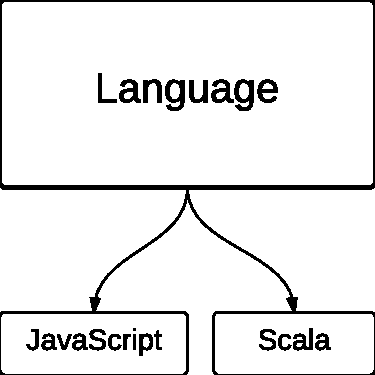
\includegraphics[width=3cm]{fat.pdf}
  \caption{Fat language}
  \label{fat-lang}
\end{figure}

\subsection{Domain Specific Languages}

Problem: interoperability.

\subsection{Thin Languages}

Alternatively, one can define concepts relative to a specific domain as libraries on top of a thin general purpose
language. Figure \ref{thin-lang} depicts this approach. The general purpose language is used as a host language that
does not need to be modified if a new concept is introduced, because concepts are defined as libraries. However,
this approach gives no opportunity to translate a concept efficiently, according to the host platform
characteristics.

\begin{figure}
  \centering
  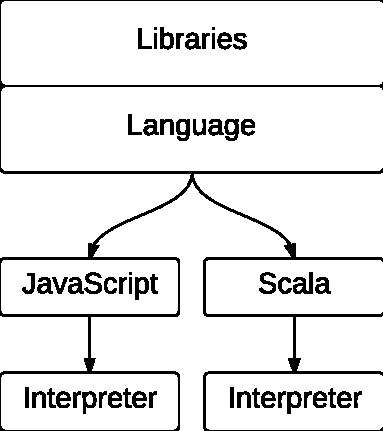
\includegraphics[width=3cm]{thin.pdf}
  \caption{Thin language}
  \label{thin-lang}
\end{figure}

\subsection{Deeply Embedded Languages}

Figure \ref{dedsl} shows a last approach that tries to get the benefits of the previous two approaches, without
their shortcomings.

\begin{figure}
  \centering
  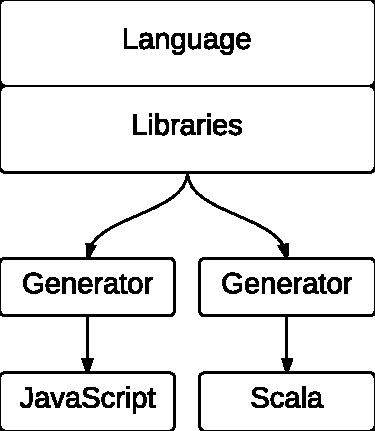
\includegraphics[width=3cm]{lms.pdf}
  \caption{Deeply embedded languages}
  \label{dedsl}
\end{figure}

Lightweight Modular Staging~\cite{Rompf12_LMSThesis} is a framework for defining deeply embedded DSLs in Scala. It
has been used to define high-performance DSLs for parallel computing~\cite{Brown11_Parallel} and can be used to
generate JavaScript code~\cite{Kossakowski12_JsDESL}.

\section{High-Level Abstractions Generating Efficient (and Heterogeneous) Code}
\label{contribution}

\subsection{Selectors}

In a Web application, the user interface is defined by a HTML document which can be manipulated by the JavaScript
code to be updated. One typical operation consists in searching some “interesting” element in the document, in order
to extract its content, replace it or listen to user events fired on this element. The standard API provides several
function to search elements in a Web document according to their characteristics such as their attribute values.
Figure~\ref{selectors-api} (wrong reference number) summarizes the available functions and their differences.

\begin{figure}
\label{selectors-api}
\begin{tabular}{| l | p{3cm} |}
\hline
Function & Description \\
\hline
\code{querySelector(s)} & First element matching the CSS selector \code{s} \\
\hline
\code{getElementById(i)} & Element which attribute \code{id} equals to \code{i} \\
\hline
\code{querySelectorAll(s)} & All nodes matching the CSS selector \code{s} \\
\hline
\code{getElementsByTagName(n)} & All elements of type \code{n} \\
\hline
\code{getElementsByClassName(c)} & All elements which \code{class} attribute equals to \code{c} \\
\hline
\end{tabular}
\caption{Standard selectors API}
\end{figure}

The \code{querySelector} and \code{querySelectorAll} are the most general functions, the others handle special
cases. For the developer it is not convenient to have to master several functions performing similar tasks. In fact,
most JavaScript developers use the jQuery library (ref and stats) that provides just one function to search for
elements. Listing~\ref{jquery-vanilla-api} shows two equivalent snippets of code, the first one using the native
APIs (a) and the second one using jQuery (b).

\begin{figure}
\begin{lstlisting}[language=JavaScript]
function getWords() {
  var form = document.getElementById('add-user');
  var sections =
    form.getElementsByTagName('fieldset');
  var results = [];
  for (var i = 0 ; i < sections.length ; i++) {
    var words = sections[i]
      .getElementsByClassName('word');
    results[i] = words;
  }
  return results
}
\end{lstlisting}
\caption{(a)}
\begin{lstlisting}
function getWords() {
  var form = $('#add-user');
  var sections = $('fieldset', form);
  return sections.map(function () {
    return $('.word', this)
  })
}
\end{lstlisting}
\caption{(b)}
\label{jquery-vanilla-api}
\end{figure}

jQuery provides an API that is simpler to master because it has less functions, but by doing so it can not benefit
from the performance of the browser’s implementation of specialized search functions (\code{getElementById},
\code{getElementsByTagName} and \code{getElementsByClassName}).

Using LMS we are able to provide a simple API (like jQuery) and to generate code using specialized functions (and
hence benefit from their performances), by analyzing the staged program. Listing~\ref{js-scala-selectors} shows how
to implement listing~\ref{jquery-vanilla-api} using js-scala. This listing generates a JavaScript program similar to
listing~\ref{jquery-vanilla-api} (a).

\begin{figure}
\label{js-scala-selectors}
\begin{lstlisting}
def getWords() = {
  val form = document.find("#add-user")
  val sections = form.findAll("fieldset")
  sections map (_.findAll(".word"))
}
\end{lstlisting}
\caption{Selectors in Js-Scala}
\end{figure}

Writing the program with js-scala instead of using a JavaScript library such as jQuery is interesting because the
abstraction for searching elements exist only in the initial program source code, not in the final JavaScript
program. It gives two advantages: (1) the execution of the final program is more performant because of the use of
specialized APIs, (2) the final program’s size is smaller because it does not need to include jQuery.

\subsection{Monads Sequencing}

As another illustration of the staging mechanism, we present a simple DSL to handle null references. This DSL
provides an abstraction at the stage-level that is removed by optimization during the code generation.

Null references are a known source of problems in programming languages~\cite{Hoare09_Null,Nanda09_Null}. For
example, consider the following typical JavaScript code finding a particular widget in the page and then a particular
button in the widget:

\begin{lstlisting}[language=JavaScript,label=null-unsafe,caption=Unsafe code]
var loginWidget =
  document.querySelector("div.login");
var loginButton =
  loginWidget.querySelector("button.submit");
loginButton.addEventListener("click", handler);
\end{lstlisting}

The native \code{querySelector} method returns \code{null} if no node matched the given selector in the document. If
we run the above code in a page where the widget is not present, it will throw an error and stop further JavaScript
execution. We can write defensive code to handle \code{null} cases, but it leads to very cumbersome code:

\begin{lstlisting}[language=JavaScript,label=null-defensive,caption=Defensive programming to handle null references]
var loginWidget =
  document.querySelector("div.login");
if (loginWidget !== null) {
  var loginButton =
    loginWidget.querySelector("button.submit");
  if (loginButton !== null) {
    loginButton.
      addEventListener("click", handler);
  }
}
\end{lstlisting}

We want to define a DSL that has both the safety and performance of listing \ref{null-defensive} but the
expressiveness of listing \ref{null-unsafe}. We can get safety by wrapping potentially null values of type
\code{Rep[A]} in a container of type \code{Rep[Option[A]]} requiring explicit dereferencing, we can get
expressiveness by using the Scala \code{for} notation for dereferencing, and finally we can get performance by
generating code that does not actually wraps values in a container but instead checks if they are \code{null} or not
when dereferenced. The wrapping container exists only at the stage-level and is removed during the code generation.
Here is a Scala listing that uses our DSL (implementation details are given in section \ref{implementation}):

\begin{lstlisting}
for {
  loginWidget <- document.find("div.login")
  loginButton <- loginWidget.find("submit.button")
} loginButton.on(Click) { e => ... }
\end{lstlisting}

The evaluation of the above listing produces a graph of statements from which JavaScript code equivalent to
listing \ref{null-defensive} is generated.

\subsection{DOM Fragments}

\begin{figure}
\label{dom-api}
\begin{lstlisting}[language=JavaScript]
var articleUi = function (article) {
  var div = document.createElement('div');
  div.setAttribute('class', 'article');
  var span = document.createElement('span');
  var name =
    document.createTextNode(article.name + ': ');
  span.appendChild(name);
  div.appendChild(span);
  var strong = document.createElement('strong');
  var price = document.createTextNode(article.price);
  strong.appendChild(price);
  div.appendChild(strong);
  return div
};
\end{lstlisting}

\begin{lstlisting}[language=HTML]
<div class=article>
  <span>French wine: </span>
  <strong>10</strong>
</div>
\end{lstlisting}
\caption{DOM}
\end{figure}

In this section we show how we can define a template engine as an embedded DSL with minimal effort. This template
engine is statically typed and able to insert dynamic content in a safe way. It provides a powerful expression
language, requires no extra compilation step and can be used on both client-side and server-side.

Because the template engine is defined as en embedded DSL, we can reuse Scala’s constructs:

\begin{itemize}
\item a function taking some parameters and returning a DOM fragment directly models a template taking parameters and
returning a DOM fragment~;
\item the type system type-checks template definitions and template calls~;
\item the Scala language itself is the expression language~;
\item compiling a template is the same as compiling user code.
\end{itemize}

So the only remaining work consists in defining the DSL vocabulary to define DOM nodes. We provide a \code{el}
function to define a tag and any \code{String} value is considered to be a text node.

\begin{figure}
\begin{lstlisting}[label=forest,caption=DOM definition DSL]
def articleUi(article: Rep[Article]) =
    el('div, 'class -> 'article)(
        el('span)(article.name + ": "),
        el('strong)(article.price)
    )
\end{lstlisting}
\end{figure}

Listing \ref{forest} uses our DSL and generates a code equivalent to listing \ref{dom-api}. The readability has
been highly improved: nesting tags is just like nesting code blocks, HTML entities are
automatically escaped in text nodes, developers have the full computational power of Scala to inject dynamic data and
DOM fragments definitions are written using functions so they compose just as functions compose. These benefits come
with no performance loss because the DSL generates code building DOM fragments by using the native JavaScript API.

Our DSL is equivalent to a template engine with Scala as the expression language. Making it usable on both server and
client sides was surprisingly as simple as defining another code generator for the DSL, producing Scala code.

For instance, the template written in listing \ref{forest} produces the following Scala code usable on
server-side:

\begin{lstlisting}
def articleUi(article: Article) = {
  val x0 = <span>{ article.name + ": " }</span>
  val x1 = <strong>{ article.price }</strong>
  val x2 =
    <div class="article">
      {List(x0, x1)}
    </div>
  x2
}
\end{lstlisting}

We are able to tackle the code sharing issues described in the introduction because of the embdedded nature
of our DSLs: dynamic content of templates is written using embedded DSLs too, so their translation into JavaScript
and Scala is managed by their respective code generators.

\subsection{Ad-Hoc Polymorphism}

Because of the dynamically typed nature of JavaScript, when calling a function there is no proper way to select a
specialized implementation according to the function’s parameters types. JavaScript is only able to dispatch
according to a method receiver prototype, \eg{} if one writes \code{foo.bar()} the JavaScript runtime will look into
the prototype of the \code{foo} object for a property named \code{bar} and will call it. So, the only way to achieve
\emph{ad hoc} polymorphism on JavaScript objects consists in defining the polymorphic function on the prototypes of
the objects. However, modifying existing object prototypes is considered bad
practice~\cite{Zakas12_MaintainableJs}. Another way could consist in manually coding the dispatch logic, by
registering supported data types at the beginning of the program execution, as described in section 2.4.3
of~\cite{Abelson83_SICP}, but this solution is painful for developers and incurs a performance overhead.

We propose to achieve \emph{ad hoc} polymorphism using
typeclasses~\cite{Wadler89_AdhocPolymorphism,Odersky06_Typeclasses,Oliveira10_Typeclasses} so that it supports
retroactive extension without modifying objects prototypes. The dispatch logic is type-directed and performed by the
compiler, so there is no runtime overhead.

\begin{figure}
\begin{lstlisting}[label=polymorphism,caption=Ad hoc polymorphism using typeclasses]
// Interface
case class Show[A](show: Rep[A => Node])

// Polymorphic function
def listWidget[A](items: Rep[List[A]])
      (implicit A: Show[A]): Rep[Node] =
  el("ul")(
    for (item <- items) yield {
      el("li")(A.show(item))
    }
  )

// Type `User`
type User = Record {
  val name: String
  val age: Int
}
// Implementation of Show for a User
implicit val showUser = Show[User] { user =>
  el("span", "class"->"user")(
    user.name + "(" + user.age + " years)"
  )
}

// Main program
def main(users: Rep[List[User]]) = {
  document.body.append(listWidget(users))
}
\end{lstlisting}
\end{figure}

Listing \ref{polymorphism} demonstrates how to define a polymorphic \code{listWidget} function that returns a DOM
tree containing the representation of a list of items. The \code{Show[A]} typeclass defines how to produce a DOM tree
for a value of type \code{A}. It is used by the \code{listWidget} function to get the DOM fragments of the list
items. The listing shows how to reuse the same \code{listWidget} function to show a list of users and a list of
articles.

\section{Implementation}
\label{implementation}

See http://github.com/js-scala/js-scala.

\subsection{Selectors}

\begin{figure}
\label{selector-impl}
\begin{lstlisting}
def find(receiver: Exp[SelectorApi],
         selector: Exp[String]) =
  getConstIdentifier(selector) match {
    case Some(id) if receiver == document =>
      DocumentGetElementById(Const(id))
    case _ =>
      SelectorFind(receiver, selector)
  }
\end{lstlisting}
\caption{Selectors optimization}
\end{figure}

\subsection{DOM Fragments}

\subsection{Ad-Hoc Polymorphism}

\section{Evaluation}
\label{validation}

We implemented several applications using js-scala. We also have written several implementations of a complete
application, using different approaches to write the client and server sides, and compared the amount of code
written, the runtime performances and the ability to modularize the code and to maintain it.

\subsection{Real World Application}

Chooze.

\subsection{Several Implementations}

\subsubsection{Vanilla JavaScript}

\subsubsection{jQuery}

\subsubsection{GWT}

\subsubsection{SharpKit}

\subsubsection{Js-Scala}

\subsection{Benchmarks, Code Metrics}

\section{Conclusion, Future Work}
\label{discussion}

%\appendix
%\section{Appendix Title}
%
%This is the text of the appendix, if you need one.
%
\acks

Acknowledgments, if needed.

\bibliographystyle{abbrvnat}
\bibliography{biblio}
%\begin{thebibliography}{}
%\softraggedright
%
%\bibitem[Smith et~al.(2009)Smith, Jones]{smith02}
%P. Q. Smith, and X. Y. Jones. ...reference text...
%
%\end{thebibliography}
%
\end{document}
